
\section{Modulación y demodulación en banda base y banda pasante}

\subsection{Caracterización de las modulaciones}

Se implementaron esquemas de modulación M-FSK, para
$M \in \{2,4,8,16\}$, y M-QAM cuadrada, para
$M \in \{4,16\}$. En ambos casos, cada símbolo representa
$k=\log_2(M)$ bits de información.

La energía de un símbolo se calcula a partir de sus componentes
en una base ortonormal:

\begin{equation}
    E(s_i)=\|\mathbf{s}_i\|^2.
\end{equation}

La energía media por símbolo y la energía media por bit se
definen como

\begin{equation}
    \overline{E}_s =
    \sum_{i=1}^{M} P(s_i)\|\mathbf{s}_i\|^2,
    \qquad
    \overline{E}_b =
    \frac{\overline{E}_s}{\log_2(M)}.
\end{equation}

Para la caracterización teórica se consideran símbolos
equiprobables y la normalización $E_b=1$. En consecuencia,
$E_s=\log_2(M)$.

La Tabla~\ref{tab:modulaciones} resume las características
de las modulaciones implementadas. Las expresiones de
probabilidad de error corresponden a un canal AWGN con
detección coherente.

\begin{table}[htbp]
    \centering
    \renewcommand{\arraystretch}{1.5}
    \begin{tabular}{|c|c|c|c|c|}
        \hline
        Modulación & $M$ & $E_s$ & $E_b$ & Dimensión \\
        \hline
        FSK & 2  & 1 & 1 & 2 \\
        FSK & 4  & 2 & 1 & 4 \\
        FSK & 8  & 3 & 1 & 8 \\
        FSK & 16 & 4 & 1 & 16 \\
        \hline
        QAM & 4  & 2 & 1 & 2 \\
        QAM & 16 & 4 & 1 & 2 \\
        \hline
    \end{tabular}
    \centering
    \caption{Caracterización teórica de las modulaciones implementadas.}
    \label{tab:modulaciones}
    \small
\end{table}

Para M-QAM cuadrada, la probabilidad teórica de error
de símbolo es

\begin{equation}
    P_s^{\mathrm{QAM}} =
    1-
    \left[
        1-
        2\left(1-\frac{1}{\sqrt{M}}\right)
        Q\left(
            \sqrt{
                \frac{3\log_2(M)}{M-1}
                \frac{E_b}{N_0}
            }
        \right)
    \right]^2,
    \label{eq:ser_qam}
\end{equation}

donde $Q(\cdot)$ representa la función de cola de la
distribución normal estándar.

Para un etiquetamiento Gray, la probabilidad de error
de bit puede aproximarse, a relaciones señal-ruido
suficientemente altas, mediante

\begin{equation}
    P_b^{\mathrm{QAM}} \approx
    \frac{4}{\log_2(M)}
    \left(1-\frac{1}{\sqrt{M}}\right)
    Q\left(
        \sqrt{
            \frac{3\log_2(M)}{M-1}
            \frac{E_b}{N_0}
        }
    \right).
    \label{eq:ber_qam}
\end{equation}

Para esta aplicación de M-FSK la probabilidad de error de símbolo puede definirse como:

\begin{equation}
    P_s^{\mathrm{FSK}}
    \approx
    (M-1)
    Q\left(\sqrt{\frac{E_s}{N_0}}\right).
    \label{eq:ser_fsk_aprox}
\end{equation}

Dado que en M-FSK ortogonal todos los símbolos se
encuentran a la misma distancia entre sí, y suponiendo
símbolos equiprobables, la probabilidad de error de bit
es

\begin{equation}
    P_b^{\mathrm{FSK}} =
    \frac{M}{2(M-1)}P_s^{\mathrm{FSK}}.
    \label{eq:ber_fsk}
\end{equation}

En la implementación de QAM se utiliza codificación
Gray, de modo que los símbolos vecinos horizontal o
verticalmente difieren en un único bit. Esta asignación
reduce la cantidad de bits incorrectos cuando el ruido
provoca una decisión hacia un símbolo vecino. Por lo
tanto, permite disminuir la probabilidad de error de bit
sin modificar la geometría de la constelación ni la
probabilidad de error de símbolo.

\subsection{Constelación de símbolos en el transmisor}

Se seleccionó la modulación 16-QAM para analizar la
constelación de símbolos generada en el transmisor.

En este esquema, cada símbolo representa cuatro bits
y se expresa mediante un vector bidimensional cuyas
componentes corresponden a los ejes en fase (I) y en
cuadratura (Q).

La constelación está formada por 16 puntos distribuidos
en una grilla de $4\times4$, con cuatro niveles de
amplitud posibles en cada eje. La separación entre
niveles se establece mediante el factor

\begin{equation}
    d =
    \sqrt{\frac{6\log_2(M)}{M-1}}.
\end{equation}

Para $M=16$, resulta

\begin{equation}
    d = \sqrt{\frac{24}{15}}
      = \sqrt{\frac{8}{5}}.
\end{equation}

Los niveles de cada componente son

\begin{equation}
    \left\{
        -\frac{3d}{2},
        -\frac{d}{2},
        \frac{d}{2},
        \frac{3d}{2}
    \right\}.
\end{equation}

En la Figura~\ref{fig:constelacion_16qam} se presenta
la constelación ideal utilizada por el transmisor,
incluyendo las etiquetas binarias asignadas a cada
punto y sus regiones de decisión.

\begin{figure}[htbp]
    \centering
    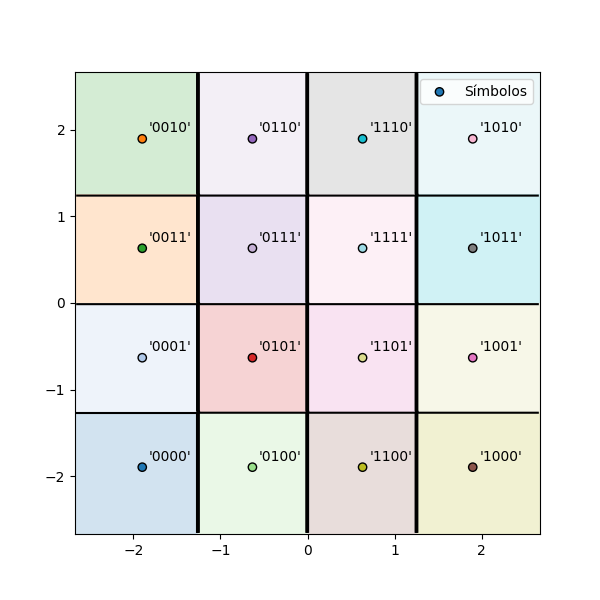
\includegraphics[width=0.6\textwidth]{../figuras/QAM.png}
    \caption{Constelación ideal de la modulación 16-QAM
    utilizada en el transmisor, con etiquetamiento Gray
    y regiones de decisión.}
    \label{fig:constelacion_16qam}
\end{figure}

La disposición de los símbolos permite transmitir
cuatro bits por cada uso del canal. En ausencia de
ruido y otras perturbaciones, cada vector transmitido
coincide exactamente con uno de los puntos de la
constelación.

\subsection{Distribución de los símbolos modulados}

Para estudiar la distribución de los símbolos
transmitidos, se utilizó el texto de Shakespeare
como fuente de información. El texto fue codificado
mediante Huffman y la secuencia binaria resultante
se agrupó en bloques de cuatro bits para realizar
la modulación 16-QAM.

El archivo contiene $5\,436\,475$ caracteres y la
codificación de Huffman produjo $25\,174\,699$ bits.
Se agregó un bit de relleno para completar el último
bloque, obteniéndose un total de $6\,293\,675$
símbolos modulados.

La Figura~\ref{fig:histograma_16qam} muestra la
cantidad de ocurrencias de cada símbolo, junto con
una escala de probabilidad. La línea de referencia
indica la frecuencia esperada bajo la hipótesis
de equiprobabilidad.

\begin{figure}[htbp]
    \centering
    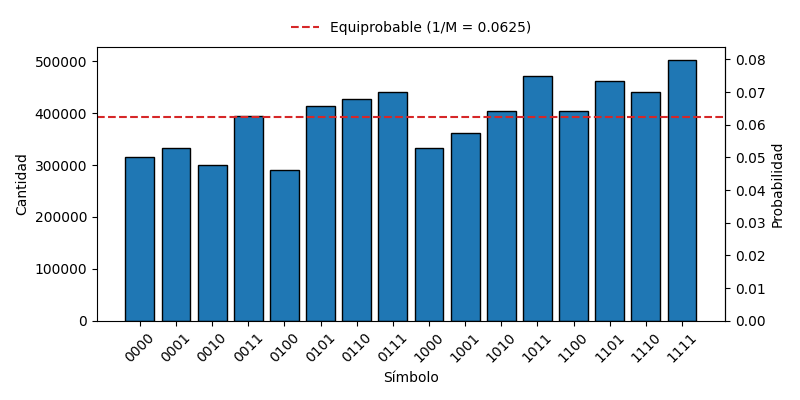
\includegraphics[width=0.7\textwidth]{../figuras/hist_QAM_16.png}
    \caption{Histograma de los símbolos transmitidos
    mediante 16-QAM a partir del texto de Shakespeare
    codificado con Huffman. La línea discontinua
    representa la frecuencia esperada para símbolos
    equiprobables.}
    \label{fig:histograma_16qam.png}
\end{figure}

Si los símbolos fueran equiprobables, cada uno
presentaría una probabilidad

\begin{equation}
    P(s_i)=\frac{1}{M}=\frac{1}{16}=0.0625.
\end{equation}

Sin embargo, los resultados experimentales muestran
diferencias apreciables entre las frecuencias de
ocurrencia. Por ejemplo, el símbolo \texttt{1111}
presentó $502\,235$ ocurrencias, con una probabilidad
estimada de $0.079800$, mientras que el símbolo
\texttt{0100} presentó $290\,005$ ocurrencias, con
una probabilidad estimada de $0.046079$.

En consecuencia, \textbf{no resulta adecuado suponer
que los símbolos transmitidos son equiprobables}
para esta secuencia particular.

Esta diferencia se debe a que la codificación de
Huffman genera una secuencia binaria cuya distribución
de bloques de cuatro bits no es necesariamente
uniforme. Aunque Huffman reduce la redundancia de la
fuente, no garantiza que todos los patrones binarios
de longitud fija tengan igual probabilidad.

\subsection{Energías medias de símbolo y de bit}

La energía media teórica de la constelación 16-QAM
se obtiene suponiendo que los 16 símbolos son
equiprobables. Con la normalización implementada,
resulta

\begin{equation}
    E_s^{\mathrm{teo}}=\log_2(16)=4,
\end{equation}

y, por lo tanto,

\begin{equation}
    E_b^{\mathrm{teo}}=
    \frac{E_s^{\mathrm{teo}}}{4}=1.
\end{equation}

Para estimar estas energías a partir de la secuencia
transmitida, se calculó la norma cuadrática de cada
vector modulado y luego se promedió sobre los $N$
símbolos generados:

\begin{equation}
    \widehat{E}_s =
    \frac{1}{N}
    \sum_{i=1}^{N}
    \|\mathbf{s}_i\|^2.
    \label{eq:energia_simbolo_estimada}
\end{equation}

La energía media estimada por bit se obtuvo como

\begin{equation}
    \widehat{E}_b =
    \frac{\widehat{E}_s}{\log_2(M)}.
    \label{eq:energia_bit_estimada}
\end{equation}

La Tabla~\ref{tab:energias_16qam} compara los
resultados teóricos y estimados para la modulación
seleccionada.

\begin{table}[htbp]
    \centering
    \caption{Comparación de energías medias teóricas
    y estimadas para 16-QAM.}
    \label{tab:energias_16qam}
    \begin{tabular}{|c|c|c|}
        \hline
        Magnitud & Valor teórico & Valor estimado \\
        \hline
        Energía media por símbolo $E_s$ & 4.0000 & 3.7637 \\
        \hline
        Energía media por bit $E_b$ & 1.0000 & 0.9409 \\
        \hline
    \end{tabular}
\end{table}

La energía media por símbolo estimada resultó
aproximadamente un $5.91\,\%$ inferior al valor
teórico calculado bajo equiprobabilidad.

Esta diferencia es consistente con el histograma
obtenido en el apartado anterior: la secuencia
transmitida no utiliza todos los puntos de la
constelación con la misma frecuencia.

En particular, los símbolos de 16-QAM presentan
distintas energías según su posición en la
constelación. Por lo tanto, una distribución no
uniforme de sus probabilidades modifica el
promedio de energía respecto del caso equiprobable.

Los resultados muestran que la normalización de
la constelación garantiza $E_b=1$ bajo la hipótesis
de símbolos equiprobables, pero no necesariamente
para una secuencia de datos con distribución
no uniforme.


\section{Efectos del canal}

En esta etapa se simularon los efectos introducidos por el canal
de comunicaciones sobre los símbolos modulados. Se consideraron
dos fenómenos: ruido blanco gaussiano aditivo (AWGN) y atenuación
aleatoria de la señal.

El modelo utilizado para representar el canal es

\begin{equation}
    \mathbf{r}_i = a_i \mathbf{s}_i + \mathbf{n}_i,
    \label{eq:modelo_canal}
\end{equation}

donde $\mathbf{s}_i$ representa el símbolo transmitido,
$a_i$ es el coeficiente de atenuación, $\mathbf{n}_i$
es el vector de ruido y $\mathbf{r}_i$ es el símbolo recibido.

\subsection{Generación de ruido AWGN}

Se implementó una función que genera muestras aleatorias
de ruido blanco gaussiano aditivo, con distribución normal
de media nula y varianza $N_0/2$ por componente.

Cada componente del vector de ruido satisface

\begin{equation}
    n_j \sim \mathcal{N}\left(0,\frac{N_0}{2}\right).
\end{equation}

Por lo tanto, el desvío estándar utilizado para generar
las muestras es

\begin{equation}
    \sigma = \sqrt{\frac{N_0}{2}}.
\end{equation}

El ruido se genera de manera independiente para cada
componente de los símbolos transmitidos y posteriormente
se suma a la señal atenuada.

\subsection{Atenuación aleatoria del canal}

Para representar las variaciones de amplitud introducidas
por el canal, se generaron coeficientes de atenuación
aleatorios con distribución uniforme en el intervalo
$[0.5,0.9]$:

\begin{equation}
    a_i \sim \mathcal{U}(0.5,0.9).
\end{equation}

Cada coeficiente multiplica las componentes del símbolo
correspondiente, reduciendo su amplitud sin modificar
su dirección en el espacio de señales.

\subsection{Aplicación de los efectos del canal}

La transmisión se simuló aplicando, para cada símbolo,
un coeficiente de atenuación y sumando posteriormente
un vector de ruido AWGN.

De esta manera, el símbolo recibido se calcula como

\begin{equation}
    \mathbf{r}_i = a_i \mathbf{s}_i + \mathbf{n}_i.
\end{equation}

La atenuación modifica la amplitud de los símbolos,
mientras que el ruido introduce desplazamientos
aleatorios en sus componentes.

La combinación de ambos efectos puede provocar que
un símbolo recibido se ubique fuera de su región
de decisión original y sea interpretado como otro
símbolo durante la demodulación.

\subsection{Constelación recibida para 16-QAM}

Para analizar los efectos del canal se utilizó la
modulación 16-QAM seleccionada en el apartado anterior.

Se consideró una relación señal-ruido de

\begin{equation}
    \frac{E_b}{N_0} = 6\,\mathrm{dB}.
\end{equation}

En escala lineal, esta relación corresponde a

\begin{equation}
    \left(\frac{E_b}{N_0}\right)_{\mathrm{lin}}
    = 10^{6/10} \approx 3.981.
\end{equation}

Considerando la energía nominal por bit $E_b=1$,
se obtiene

\begin{equation}
    N_0 = \frac{1}{10^{6/10}} \approx 0.2512.
\end{equation}

En la Figura~\ref{fig:constelacion_canal_16qam}
se presenta la constelación recibida luego de aplicar
la atenuación y el ruido AWGN.

\begin{figure}[htbp]
    \centering
    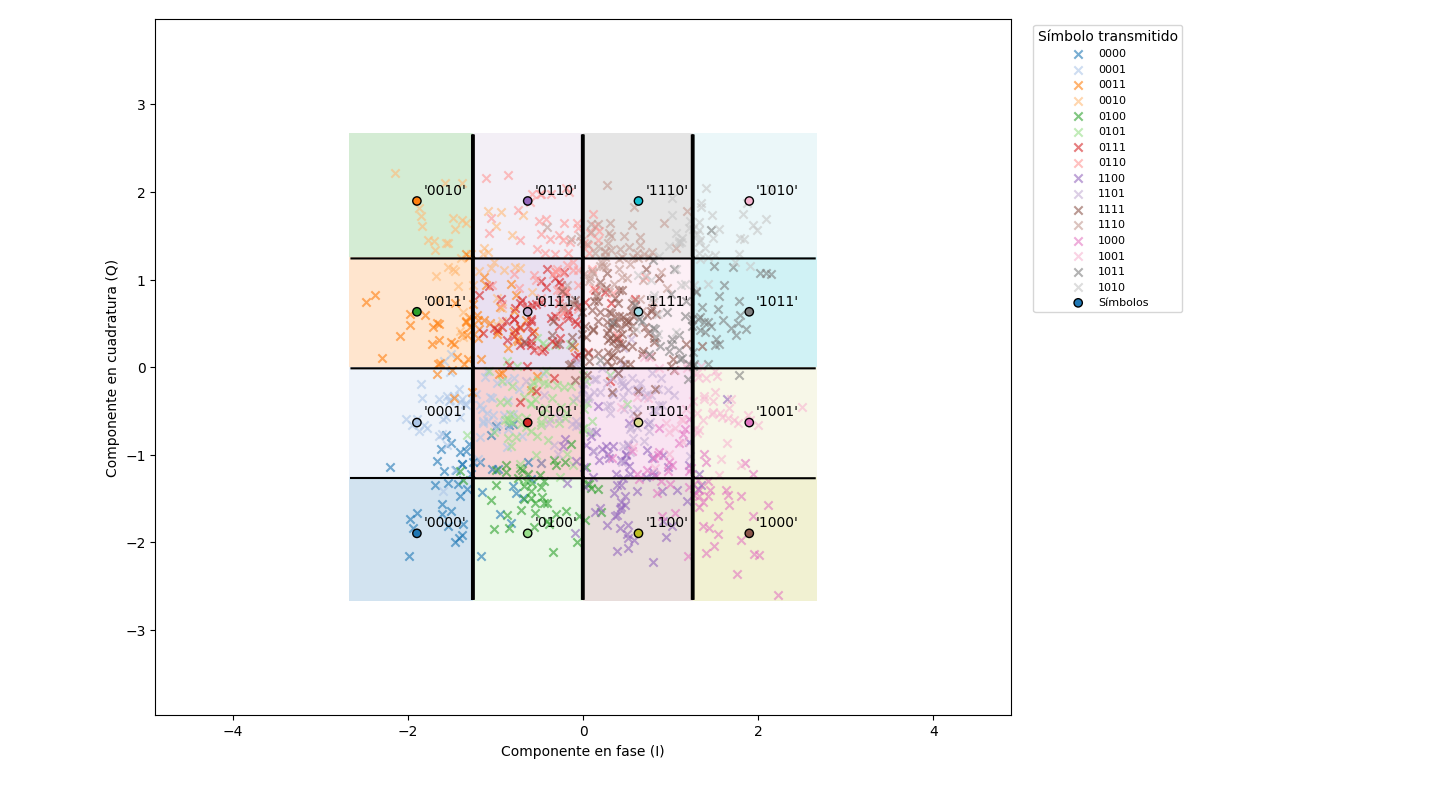
\includegraphics[width=0.8\textwidth]{../figuras/QAM_RUIDO.png}
    \caption{Constelación 16-QAM recibida para
    $E_b/N_0=6\,\mathrm{dB}$, considerando atenuación
    uniforme entre 0.5 y 0.9 y ruido AWGN.
    Los colores de las muestras identifican
    los símbolos originalmente transmitidos.}
    \label{fig:constelacion_canal_16qam}
\end{figure}

En el gráfico, cada símbolo transmitido se representa
mediante un color diferente. Las cruces corresponden
a las muestras recibidas, mientras que los puntos
de la constelación ideal y sus etiquetas binarias
permiten identificar las posiciones de referencia.

Esta representación permite distinguir las muestras
asociadas a cada símbolo transmitido, incluso cuando
el ruido y la atenuación las desplazan hacia otras
regiones de decisión.

Se observa que la atenuación produce una contracción
de la constelación hacia el origen, mientras que
el ruido AWGN genera una dispersión aleatoria
alrededor de las posiciones atenuadas.

Como consecuencia, algunas muestras pueden atravesar
las fronteras de decisión correspondientes a otros
símbolos, produciendo posibles errores de detección.

La visualización mediante colores facilita el análisis
de estos desplazamientos, ya que permite reconocer
el símbolo de origen independientemente de la región
en la que finalmente se encuentra la muestra recibida.

